\chapter{VisioneImpresa}\label{chap:VisioneImpresa}

\section{L'azienda}
{\company} è un'azienda con quarant'anni di esperienza nell'offrire a piccole e medie imprese soluzioni informatiche per la 
gestione e l'automazione dei processi aziendali. I suoi prodotti di punta sono infatti sistemi \gls{erp} (\textit{Enterprise 
Resource Planning}) ovvero sistemi che permettono di coordinare il flusso di dati tra i processi di un'azienda, fornendo un'unica fonte di 
informazioni e semplificandone le operazioni.\\
{\company} è situata a Pernumia (Padova) e opera in prevalenza nel Nord Est, dal 2016 è entrata a far parte del gruppo Officegroup, azienda 
che riunisce diverse \textit{software house} specializzate nella progettazione e sviluppo di sistemi gestionali evoluti. 
Dal 2023 inoltre è diventata una società \textit{benefit}, ovvero è un azienda che opera con l'obiettivo di generare un impatto positivo 
sulla società e sull'ambiente, oltre al profitto finanziario.

\begin{figure}[H]
    \centering
    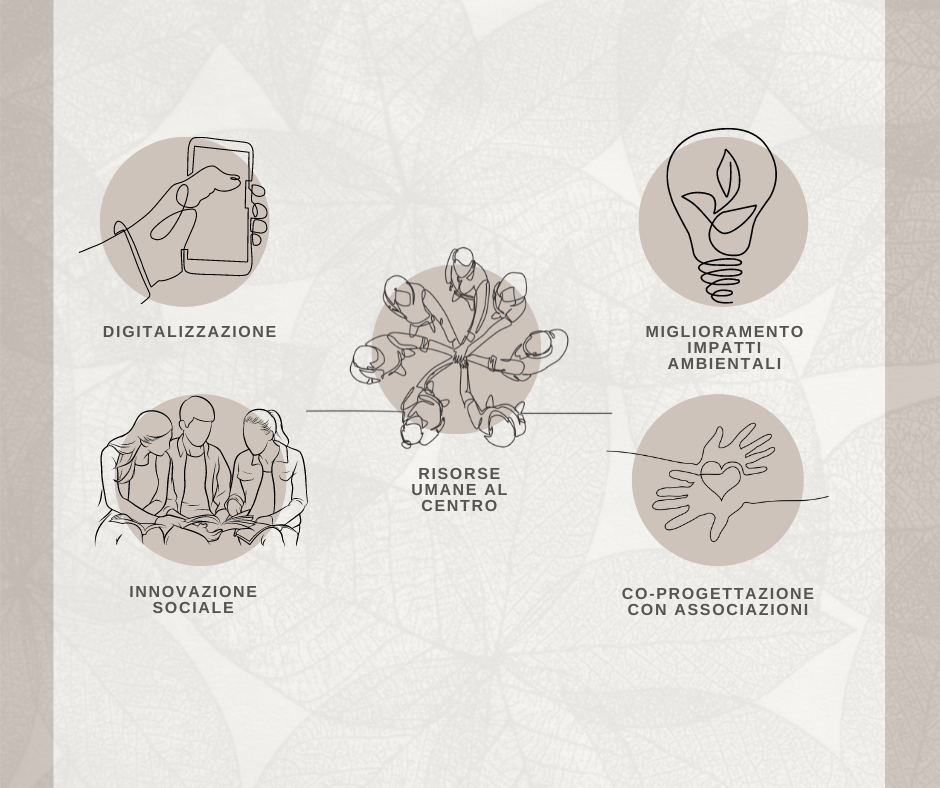
\includegraphics[alt={Obiettivi delle società benefit}, width=0.5\textwidth]{img/soc-benefit.png}
    \caption[Obiettivi delle società benefit.]{Obiettivi delle società benefit. \\ \textit{fonte: https://www.vsh.it/azienda/societa-benefit/}}
    \label{fig:società benefit}
\end{figure}

Come mostrato in Figura \ref{fig:società benefit} questo tipo di società attuano iniziative in diversi ambiti, dalla dematerializzazione 
e digitalizzazione alla promozione di politiche a sostegno della conciliazione vita-lavoro.\\
Altri obiettivi delle società \textit{benefit} possono essere: investire nelle \textbf{energie rinnovabili e la sostenibilità}, l'investimento in \textbf{tecnologie 
ad alta efficienza energetica}, rispetto della \textbf{parità di genere}, \textbf{formazione professionale} del lavoratore, \textbf{progetti con scuole ed 
università, co-progettazione con associazioni e istituzioni del territorio} con il duplice obiettivo di stimolare la partecipazione dei dipendenti 
a “buone cause” della comunità e \textbf{valorizzare il lavoro di associazioni no-profit} del territorio, generando così valore sociale.


\section{Clienti e servizi}
{\company} ha come clienti piccole e medie imprese situate in prevalenza in Veneto e in generale nel Nord Italia, possiamo trovare però 
anche clienti dal Centro Italia e dalla Sardegna. \\
Il gestionale che propone può adattarsi a qualsiasi tipo di azienda indipendentemente dal settore in cui 
operi (anche se come vedremo vengono venduti dei gestionali ad hoc per i settori: petrolifero, ittico, assistenza post-vendita, ortofrutticolo, antincendi 
e antinfortunistica, trasporti).\\ Una volta implementato il gestionale all'interno dell'azienda del cliente viene offerta una formazione all'utilizzo del 
\textit{software} per i dipendenti, che parteciperanno a delle riunioni tenute da un consulente tecnico che ne illustrerà le funzionalità e insegnerà come sfruttarle 
al meglio.\\
{\company} propone due linee di prodotti principali: Vision e MoviDAT.
La prima, Vision, è la linea di gestionali dell'azienda, con VisionENTERPRISE, che è il loro \gls{erp} di punta, 
e poi una serie di soluzioni verticali per venire incontro alle specifiche esigenze delle varie aziende con cui {\company} opera.
Ognuna delle soluzioni verticali offerte dall'azienda è una variazione di VisionENTERPRISE, che viene arricchita con 
funzionalità specifiche per adattarsi a specifici settori. In particolare quindi nella linea Vision abbiamo:
\begin{itemize}
      \item \textbf{VisionENTERPRISE}, \gls{erp} di punta dell'azienda e dedicato ad imprese che non hanno necessità di funzionalità 
      specifiche.
      \item \textbf{VisionENERGY}, gestionale con specifiche funzionalità pensate per le aziende che lavorano nel settore petrolifero, 
      come la possibilità di gestire la vendita di carburante, manutenzione valvole, ecc.;
      \item \textbf{VisionBLUE}, gestionale con specifiche funzionalità pensate per le aziende che lavorano nel settore ittico, 
      come la possibilità di gestire lotti, prodotti e imballaggi;
      \item \textbf{VisionASSISTANCE}, gestionale con specifiche funzionalità pensate per le aziende specializzate nell'assistenza post-vendita, 
      come la possibilità di gestire richieste di assistenza, contratti e assegnare gli ordini di intervento ai 
      singoli tecnici;
      \item \textbf{VisionFRESH}, gestionale con specifiche funzionalità pensate per le aziende che lavorano nel settore ortofrutticolo, 
      come la possibilità di gestire movimentazione merce, inserimento pesate, interfacciamento con bilance elettroniche, ecc.;
      \item \textbf{VisionANTINCENDI}, gestionale con specifiche funzionalità pensate per le aziende che lavorano nel settore antincendi e antinfortunistica, 
      come la possibilità di gestire chiamate ed interventi straordinari, buoni di manutenzione e geolocalizzare gli interventi;
      \item \textbf{VisionTRASPORTI}, gestionale con specifiche funzionalità pensate per le aziende che lavorano nel settore trasporti, 
      come la possibilità di gestire listini, anagrafiche, dotazioni, manutenzione, pianificazione viaggi, ecc.
\end{itemize}
Nella linea di prodotti MoviDAT invece troviamo una gamma di applicazioni sviluppate per i principali sistemi operativi per dispositivi 
\textit{mobile}: Android e iOS. Queste applicazioni sono state sviluppate per integrarsi direttamente con i gestionali 
della linea Vision e permettono di semplificare il lavoro di dipendenti che operano in mobilità e non hanno a disposizione un 
\textit{computer} con cui lavorare durante le trasferte (ed anche se ce lo avessero il suo utilizzo risulterebbe scomodo).\\
In questa linea dunque troviamo:
\begin{itemize}
    \item \textbf{MoviDOC} è un \gls{webapp} (ovvero un \textit{app} a cui è possibile accedere direttamente da \textit{browser} senza 
          necessità di installarla sul dispositivo) che consente la gestione e condivisone dei documenti;
    \item \textbf{Handy} è un \textit{app} per palmare che integrata a VisionENTERPRISE supporta la movimentazione della merce del magazzino o del punto vendita;
    \item \textbf{MoviSELL} è un \textit{app} sviluppata per \textit{tablet} iOS dedicata agli agenti aziendali, permette di: visualizzare i 
          clienti su una mappa, avere visibilità dello stato contabile e inserire ordini clienti direttamente nel 
          ciclo attivo dell'azienda.
    \item \textbf{MoviREP} è un \textit{app} sviluppata per \textit{tablet} iOS per la gestione digitalizzata dei rapportini da parte di operatori addetti alla manutenzione o 
          all'assistenza post vendita. 
    \item \textbf{MoviALERT} è una \gls{webapp} che permette di inviare \textit{mail} di notifica automatiche all'avvenire di 
          specifici eventi nel gestionale;
    \item \textbf{MoviCHECK} è un \gls{webapp}, scaricabile anche su dispositivi Android e iOS per 
          consultare i dati di business in mobilità;
    \item \textbf{MoviEXPENSE} è un \textit{app} per Android e iOS, per la registrazione automatica delle note 
          spese;
    \item \textbf{MoviCHECKIN} è una \gls{webapp} per la registrazione dei visitatori in azienda;
    \item \textbf{MoviORDER} applicazione per \textit{smartphone e tablet} iOS e Android che l’azienda può fornire ai propri clienti per l’invio di ordini e 
          richieste di approvvigionamento.
\end{itemize}

Nel caso in cui un'azienda richieda funzionalità specifiche per uno dei \textit{software} sopra elencati, {\company} offre la possibilità di creare una versione 
modificata dei propri prodotti. Per evitare di avere troppe variazioni della stesso prodotto il codice delle personalizzazioni (così vengono chiamate le funzioni in 
più richieste dal cliente) vengono inserite direttamente nel codice del \textit{software} principale, e "attivate" da specifici parametri controllati all'avvio del 
sistema. Nel caso di MoviORDER, che ho avuto la possibilità di esaminare per questo progetto, a seconda del valore del campo \textit{Company} ottenuto a seguito dell'
autenticazione del cliente venivano apportate alcune variazioni grafiche (loghi, tema). Questo si può ottenere grazie ad un'attenta progettazione e appropriate scelte 
architetturali.

 
\section{Organizzazione aziendale}
\subsection{Aree di competenza}
{\company} è strutturata in tre aree di competenza, ognuna con ruoli e responsabilità specifiche.\\
\textbf{Reparto Assistenza}: qui operano i consulenti tecnici gestionali, il cui compito è assistere l'azienda nell'implementazione dei nuovi gestionali 
e nella gestione del cambiamento assicurandosi che il personale aziendale sia formato sull'uso delle nuove tecnologie. Ogni consulente è responsabile di uno 
o più \textit{software} di cui hanno un ampia conoscenza operativa. Inoltre, forniscono assistenza ai clienti, aiutandoli 
nella risoluzione dei problemi e, se necessario, segnalando le problematiche al reparto sviluppo che aprirà quindi un 
\textit{ticket} all'interno della piattaforma Jira (vedi capitolo \ref{chap:Tecnologie}).\\
\textbf{Area Amministrazione Commerciale e \textit{Marketing}}: In quest'area si trovano diverse competenze, tra cui:
\begin{itemize}
    \item \textbf{Responsabile \textit{marketing}}: ha il compito di realizzare strategie per promuovere l'azienda 
          e i suoi prodotti ai potenziali clienti;
    \item \textbf{Risorse umane}: ha il compito di amministrare stipendi, pensioni e \textit{benefit}, nonché di assicurarsi il rispetto da parte 
          dell'azienda delle normative sul lavoro;
    \item \textbf{Contabilità}: ha il compito di gestire e registrare le transazioni finanziarie, garantendo che tutte le attività economiche 
          siano documentate in modo accurato e trasparente;
    \item \textbf{Segreteria generale}: ha il compito di gestire e indirizzare le chiamate in entrata, gestire la posta elettronica e la 
          corrispondenza, pianificare eventi aziendali;
    \item \textbf{Segreteria commerciale}: ha il compito di mantenere le comunicazioni con i clienti fornendo informazioni su prodotti e 
          servizi e preparando offerte commerciali, contratti di vendita e documenti correlati;
    \item \textbf{Amministrazione ciclo attivo}: ha il compito di garantire una gestione efficiente delle vendite e della riscossione dei pagamenti;
    \item \textbf{Commerciale rete diretta}: ha il compito di occuparsi della vendita dei prodotti direttamente ai clienti finali;
    \item \textbf{commerciale rete indiretta}: ha il compito di gestire le vendite attraverso intermediari come distributori, rivenditori, agenti o partner commerciali;
    \item \textbf{Responsabile d'impatto}: si occupa della valutazione, pianificazione e promozione delle misure di responsabilità sociale d'impresa 
          (\gls{csr}), ovvero di tutte le iniziative attuate dall'azienda in ambito sociale e di transizione ecologica.
    \item \textbf{Amministratore} è responsabile di dirigere e gestire l'azienda nel suo complesso, assicurando che tutti i dipartimenti e le attività 
          lavorino insieme per raggiungere gli obiettivi strategici e operativi.
    \item \textbf{\textit{Product manager}} ha il compito di assicurare che i prodotti siano sviluppati in linea con le esigenze del mercato, lanciati con
          successo e gestiti efficacemente durante il loro ciclo di vita.
\end{itemize}
\textbf{Reparto Sviluppo \textit{Software}}: In quest'area troviamo:
\begin{itemize}
    \item \textbf{Sviluppatori}: possono essere \textbf{\textit{frontend}}, specializzati nello sviluppo di interfacce e della gestione dell'
          interazione uomo-macchina, \textbf{\textit{backend}} specializzati nello sviluppo della logica del \textit{software} e nella manipolazione dei 
          dati, o \textbf{\textit{fullstack}}, in grado di operare sia come sviluppatore \textit{frontend} che \textit{backend}.
    \item \textbf{\textit{Project manager}}: ha il compito di assicurarsi che vengano rispettati obiettivi, tempi, costi e vengano soddisfatti
          i parametri di qualità;
    \item \textbf{Direttore dello sviluppo}: ha il compito di prendere le decisioni implementative e scegliere l'architettura del \textit{software}, si 
          occupa inoltre di dirigere il team e di pianificare e assegnare i lavori da svolgere;
    \item \textbf{Analista}: si occupa di interagire con i clienti per delineare i requisiti del progetto \textit{software} e documentarli in un documento 
          di analisi.
\end{itemize}

\subsection{Metodologie di sviluppo \textit{software}}
Ho potuto notare, durante la mia esperienza di tirocinio, che gli sviluppatori utilizzano metodologie Agile per la gestione dei loro progetti.\\
Le metodologie Agile sono un'approccio alla gestione dei progetti che prevede la suddivisione del progetto 
in fasi e del lavoro in cicli brevi, al termine dei quali verranno introdotti cambiamenti che avvicinano il 
progetto sempre di più al soddisfacimento di tutti i requisiti. Questo approccio è particolarmente adattabile agli imprevisti, permettendo di reagire velocemente 
e riducendo al minimo i danni, come lo slittamento della data di completamento e conseguentemente l'aumento di denaro da destinare al progetto. 
Il manifesto Agile riporta i punti principali punti di questa filosofia:
\begin{itemize}
      \item Gli \textbf{individui e le interazioni} più che i processi e gli strumenti;
      \item Il \textbf{software funzionante} più che la documentazione esaustiva;
      \item La \textbf{collaborazione col cliente} più che la negoziazione del contratto;
      \item \textbf{Rispondere al cambiamento} più che seguire un piano.
\end{itemize}
In particolare, {\company} adotta il \textit{framework} Agile Scrum, che definisce una 
serie di principi, pratiche e cerimonie per riuscire ad assimilare nel proprio metodo di lavoro la metodologia Agile. 
Scrum richiede di suddividere il lavoro in \textit{sprint} dalla durata variabile di una fino a quattro settimane. {\company} pianifica
sprint di una settima in modo da rispondere tempestivamente a gli imprevisti ed effettuare una pianificazione più efficace.

\begin{figure}[H]
      \centering
      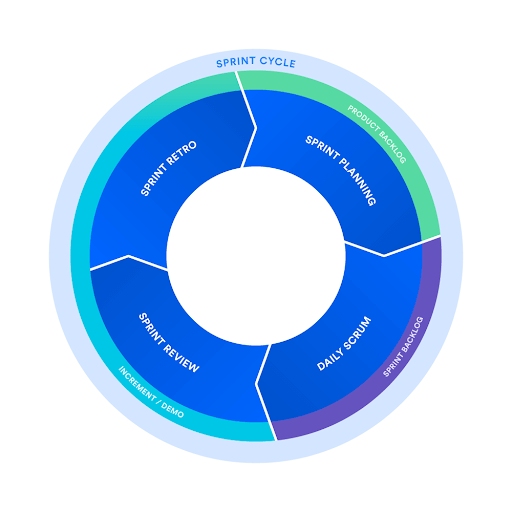
\includegraphics[alt={Organizzazione di uno sprint con il \textit{framework} Scrum}, width=0.5\textwidth]{img/scrum.png}
      \caption[Organizzazione di uno sprint con il \textit{framework} Scrum]
              {Organizzazione di uno sprint con il \textit{framework} Scrum. \\ \textit{fonte: https://www.atlassian.com/it/agile/scrum}}
      \label{fig:scrum}
  \end{figure}

Come mostrato in Figura \ref{fig:scrum} ogni sprint è strutturato in una serie di incontri che avvengono solitamente in video chiamata usando 
3CX (vedi capitolo \ref{chap:Tecnologie}).\\ 
Si comincia il lunedì, all'inizio dello \textit{sprint}, quando programmatori, direttore dello sviluppo e \textit{project manager} partecipano 
ad un \textit{meeting} chiamato \textit{sprint planning} dove si pianifica il lavoro da svolgere per lo sprint in corso.
Quindi ogni giorno si tiene un breve \textit{meeting} prima della pausa pranzo chiamato \textit{daily scrum} dove si discute dello stato dei lavori ed 
eventuali problemi emersi.
Il venerdì si tiene l'ultimo \textit{meeting} dello \textit{sprint} chiamato \textit{sprint review} dove si discute 
dello stato dei lavori rispetto alle aspettative e discutendo dei problemi emersi durante lo \textit{sprint} si cercano modi per migliorare.\\
{\company} organizza inoltre un ulteriore \textit{meeting} a cadenza mensile dove non solo le persone interessate al progetto, ma tutti i dipendenti dell'azienda 
si riuniscono per discutere dello stato dei lavori di ogni settore: \textbf{evoluzione dei prodotti, vendite, feedback dei clienti, aggiornare il reparto \textit{marketing}
 e commerciale sulle nuove funzionalità dei software ecc.}. Questo incontro ha 
lo scopo di dare a tutti i dipendenti dell'azienda una visione d'insieme evitando il cosiddetto "effetto sottomarino", ovvero quando una persona o un gruppo si focalizzano 
soltanto in uno specifico ambito, favorendo l'isolamento rispetto al resto dell'azienda, che ha invece bisogno di lavorare coordinando i vari settori.


%\begin{itemize}
%	\item gli acronimi, le abbreviazioni e i termini ambigui o di uso non comune menzionati vengono definiti nel glossario, situato alla fine del presente documento;
%	\item per la prima occorrenza dei termini riportati nel glossario viene utilizzata la seguente nomenclatura: \gls{apig};
%	\item i termini in lingua straniera o facenti parti del gergo tecnico sono evidenziati con il carattere \textit{corsivo}.
%\end{itemize}

\newpage